\section{Realisering}
Kredsløbene fra analysen og simuleringen opbygges og måles i laboratoriet med oscilloskop. Figurerne nedenfor viser de fysiske måleopstillinger. 

\begin{figure}
\begin{center}
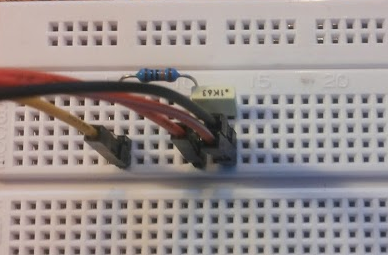
\includegraphics[height=5cm]{E_Fig/Rea_1_100}
\caption{Lavpasfilter R: 100 k$Omega$, C = 100nF
\label{Rea_1_100}
\end{center}
\end{figure}

\begin{figure}
\begin{center}
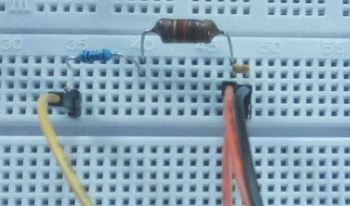
\includegraphics[height=5cm]{E_Fig/Rea_2_1}
\caption{Lavpasfilter R=1k$Omega$, =1mH, C=1nF}
\label{Rea_2_1}
\end{center}
\end{figure}

\subsection{Realisering af 1. ordens lavpasfilter}


\subsubsection{10k$Omega$}

\begin{figure}
\begin{center}
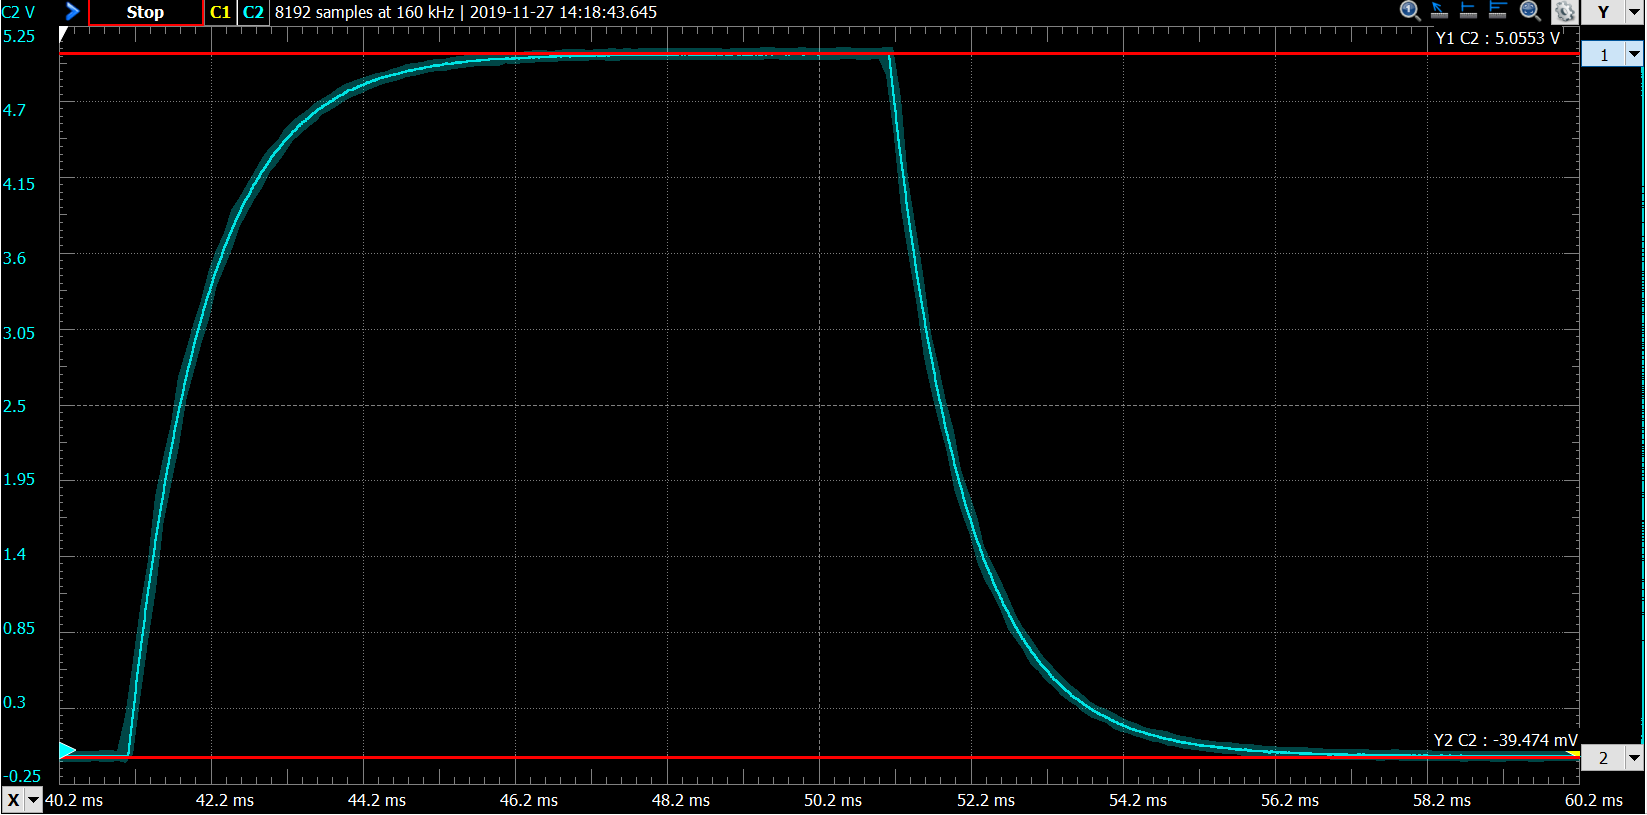
\includegraphics[height=5cm]{E_Fig/Rea_1_10_max}
\caption{Måling af $V_[max]$ på 10k$\Omega$ 1. ordens lavpasfilter}
\label{Rea_1_10_max}
\end{center}
\end{figure}

Oscilloskopet indstilles til en amplitude på 2.5V, offset på 2.5V og en frekvens på 50 Hz.$V_{max}$ måles til 5.06V

\begin{figure}
\begin{center}
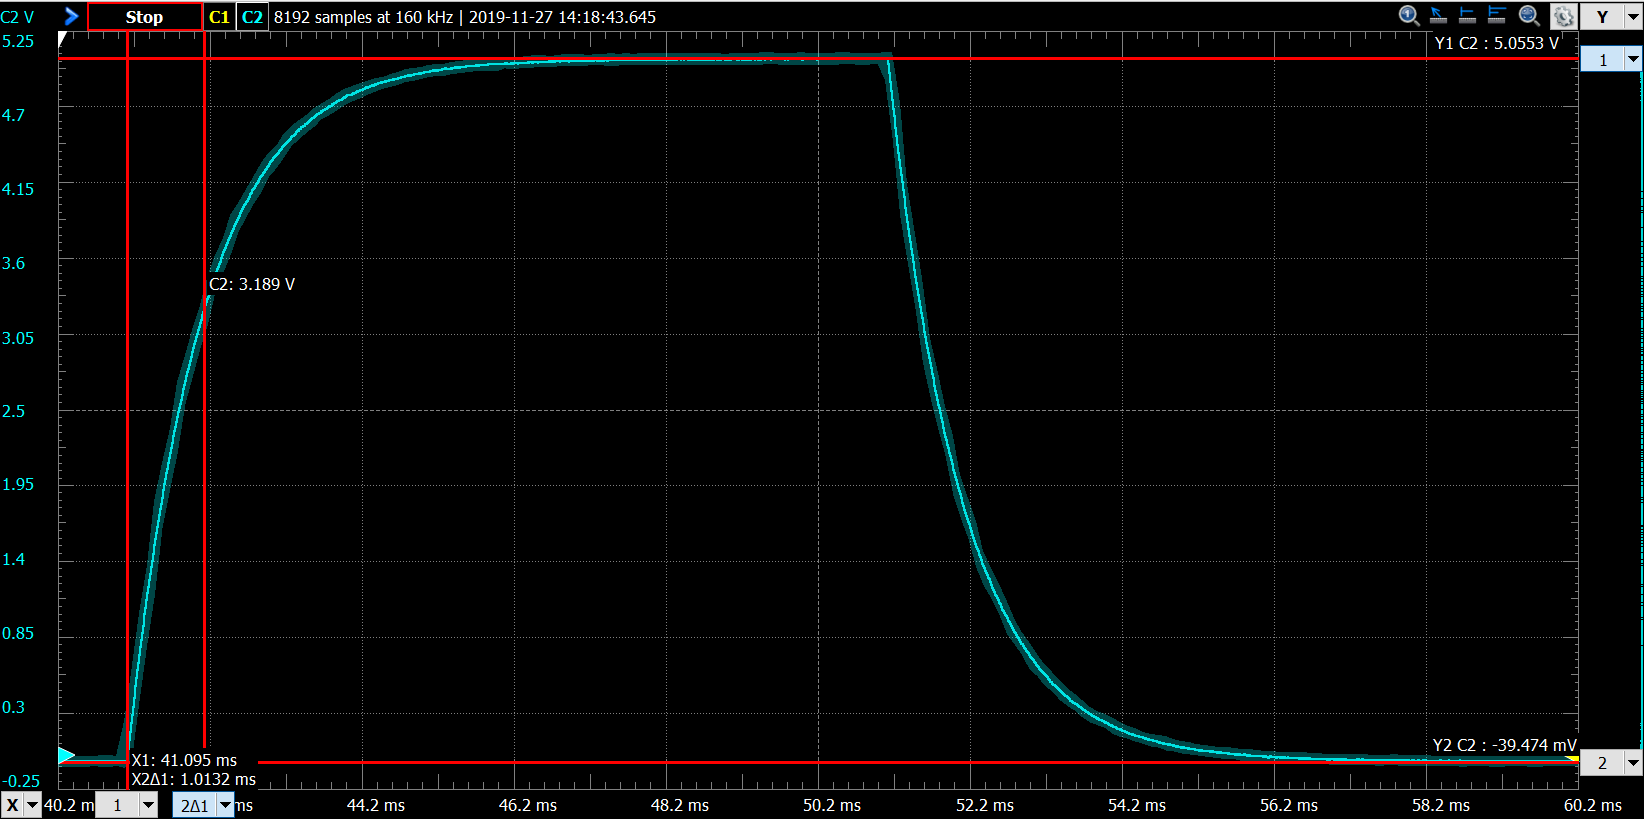
\includegraphics[height=5cm]{E_Fig/Rea_1_10_tidskonstant}
\caption{Måling af tidskonstant på 10k$\Omega$ 1. ordens lavpasfilter}
\label{Rea_1_10_tidskonstant}
\end{center}
\end{figure}

Tidskonstanten måles til 63$%$ af den stationære spænding, hvilket udregnes til $5.06V*0.63=3.188V$. Tidskonstanten $\tau$ måles her til $1.01 ms$.

\begin{figure}
\begin{center}
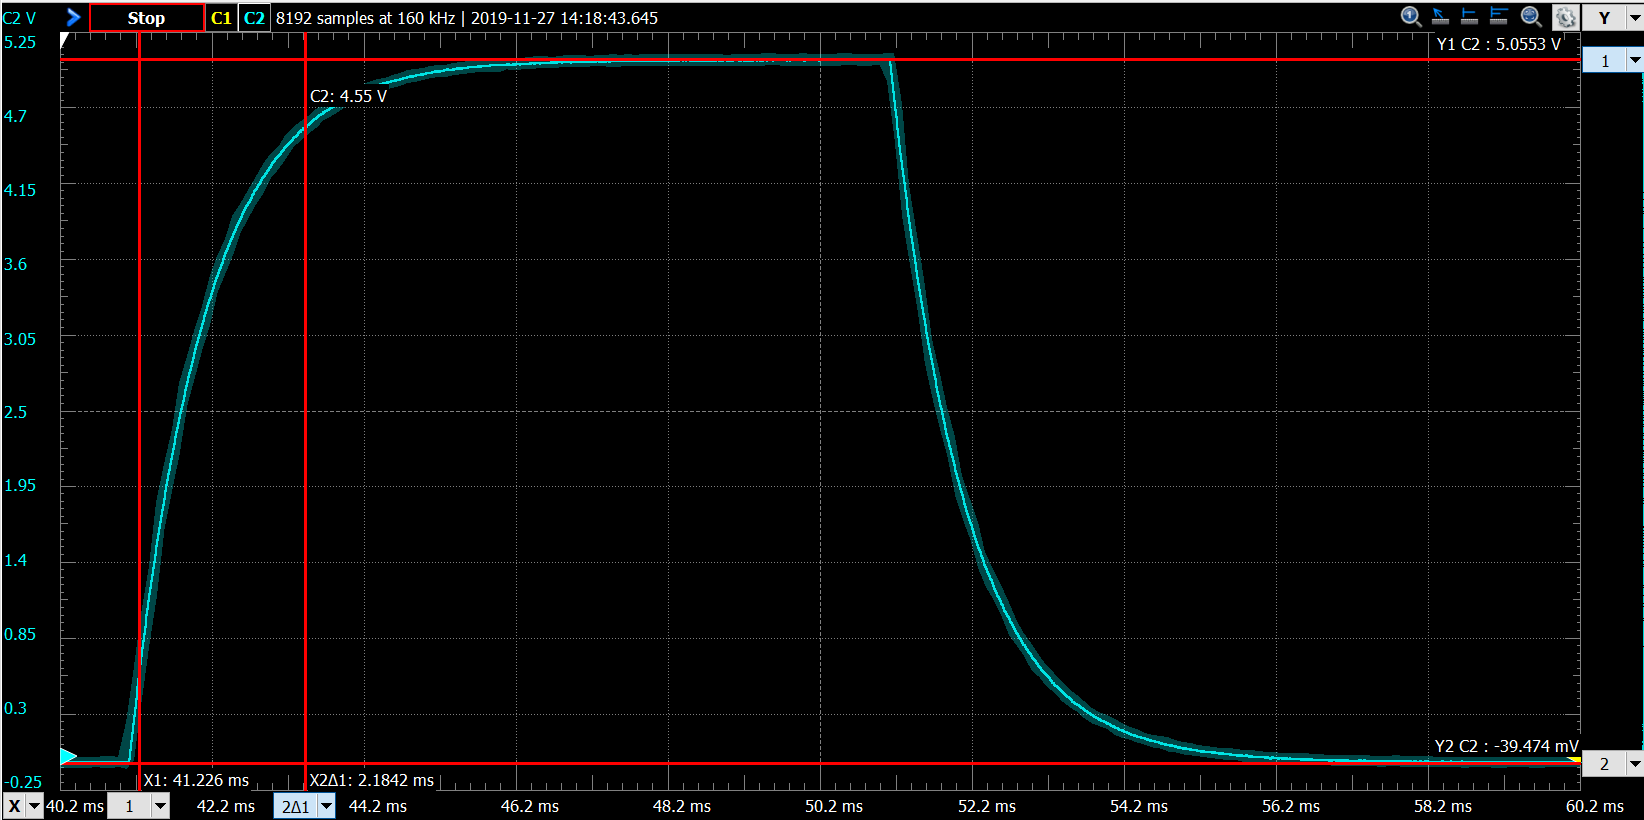
\includegraphics[height=5cm]{E_Fig/Rea_1_10_stigetid}
\caption{Måling af stigetid på 10k$\Omega$ 1. ordens lavpasfilter}
\label{Rea_1_10_stigetid}
\end{center}
\end{figure}

Stigetiden måles ved at måles tiden til 10$%$ og 90$%$ af den stationære spænding.
$t_{10}=5.06 V \cdot 0.1 = 0.506 V$
$t_{90}=5.05 V \cdot 0.9 = 4.554 V$
Stigetiden $t_r$ måles til $2.18 ms$

\subsubsection{100k$Omega$}

\begin{figure}
\begin{center}
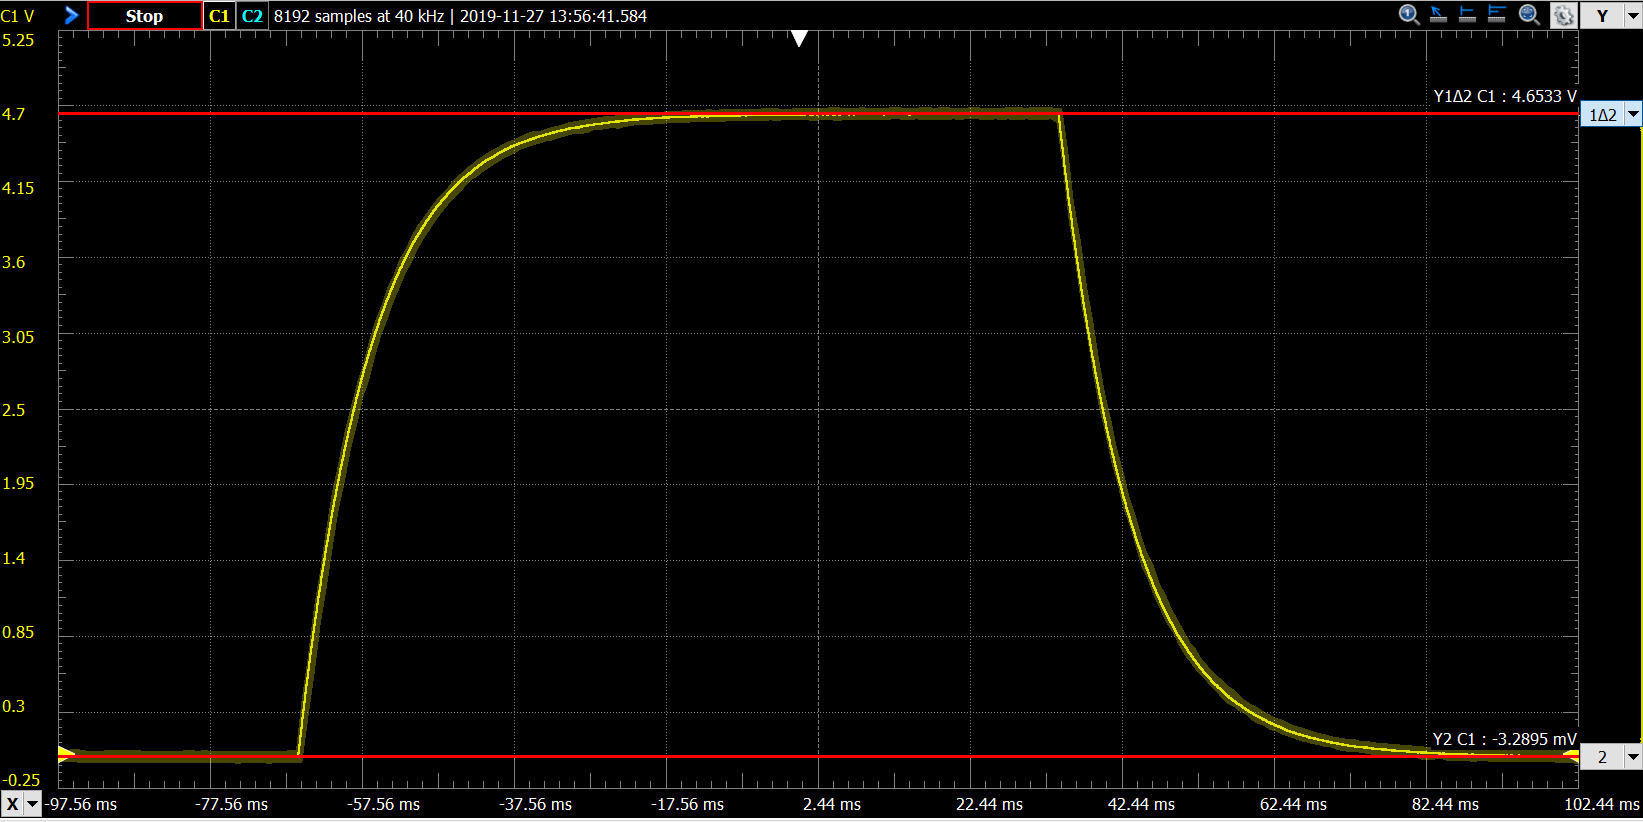
\includegraphics[height=5cm]{E_Tex/Rea_1_100_max}
\caption{Måling $V_{max}$ på 1. ordens lavpasfilter med 100k$Omega$}
\label{Rea_1_100_max}
\end{center}
\end{figure}

Oscilloskopet indstilles til en amplitude på 2.5V, et offset på 2.5 V og en frekvens på 5 Hz
$V_{max}$ måles på lavpasfilteret med en 100k$\Omega$ modstand til 4.65 V. 

\begin{figure}
\begin{center}
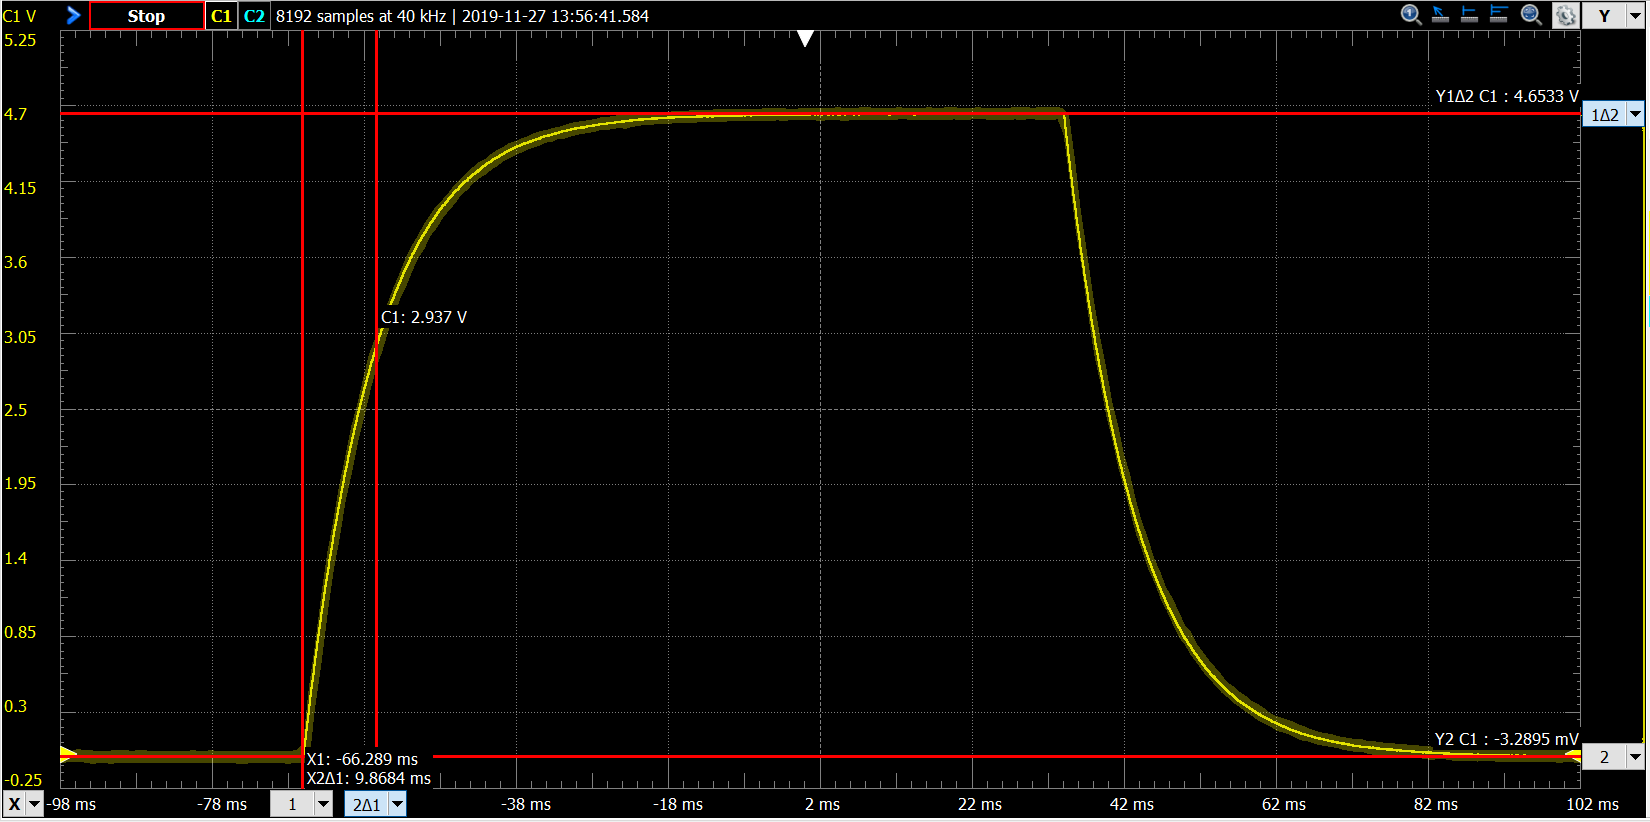
\includegraphics[height=5cm]{E_Fig/Rea_1_100_tidskonstant}
\caption{Måling af tidskonstant på 100k$\Omega$ 1. ordens lavpasfilter}
\label{Rea_1_100_tidskonstant}
\end{center}
\end{figure}

Tidskonstanten måles til 63$%$ af den aflæste maximale spænding, som svarer til den stationære spænding, hvilket er $4.65 V \cdot 0.63 = 2.93 V$. Tiden til 2.93 V, stigetiden, aflæses til 9.87 ms.

\begin{figure}
\begin{center}
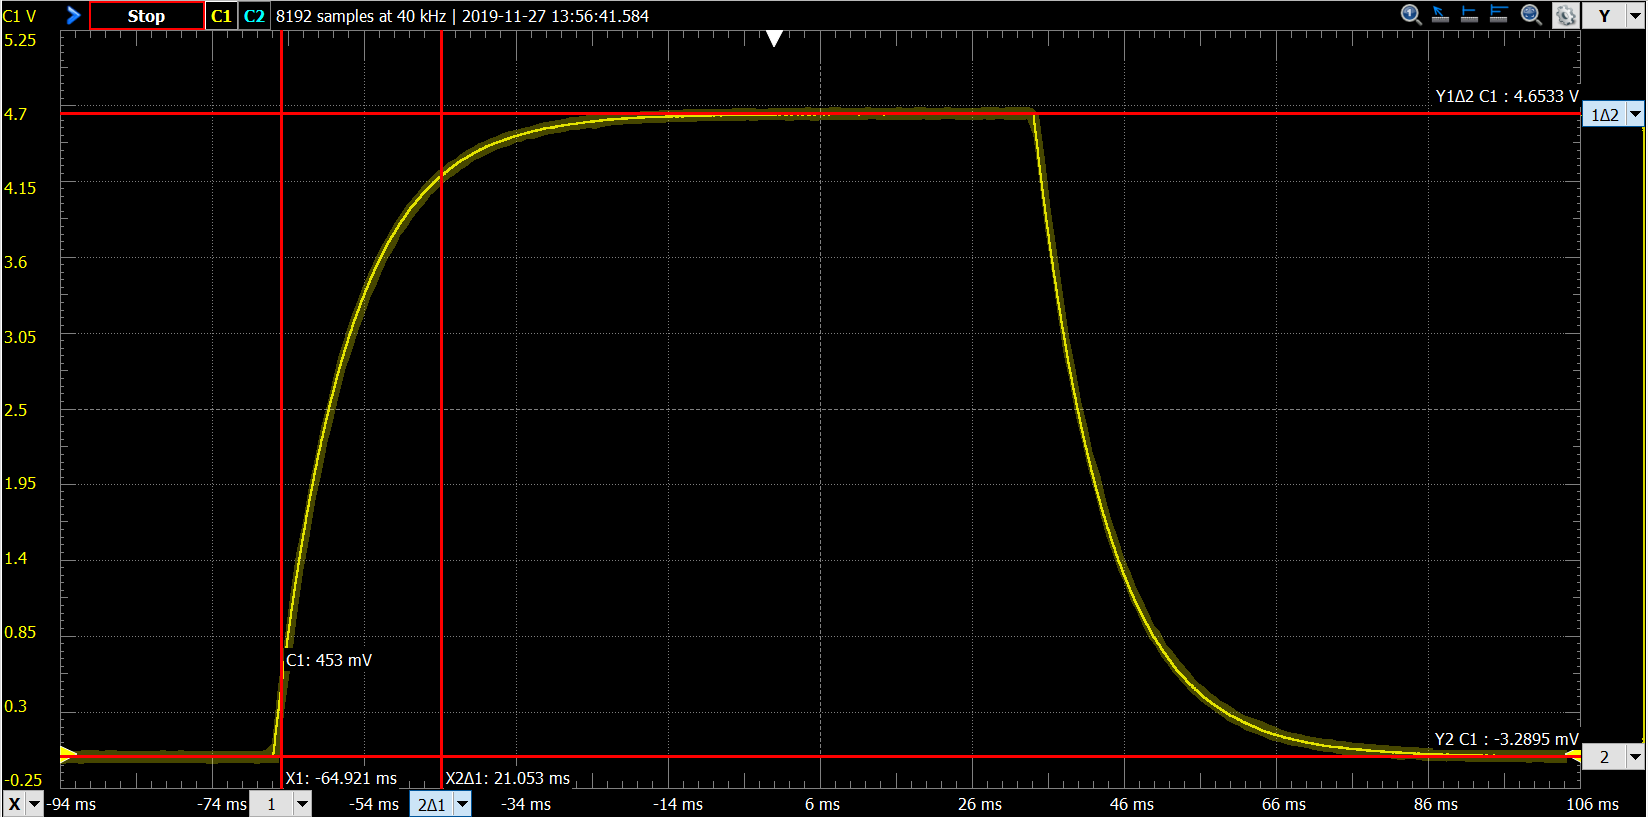
\includegraphics[height=5cm]{E_Fig/Rea_1_100_stigetid}
\caption{Måling at stigetid på 100k$\Omega$ 1. ordens lavpasfilter}
\label{Rea_1_100_stigetid}
\end{center}
\end{figure}

Stigetiden måles ved at måles tiden til 10$%$ og 90$%$ af den stationære spænding, som svarer til den aflæste maksimale spænding
.
$t_{10}=4.65 V \cdot 0.1 = 0.465 V$
$t_{90}=4.65 V \cdot 0.9 = 4.185 V$
Stigetiden $t_r$ måles til $21.05 ms$


\subsection{Realisering af 2. ordens lavpasfilter}

\subsubsection{10k$\Omega$}



\subsubsection{1k$\Omega$}